\section{Bonus: Additional feature}
\subsection{Twilio SMS API Integration}

Using the Twilio Messaging API, We can set up a cronjob which fetches any messages that have yet to be sent

\subsubsection{MySQL Query}
\begin{minted}{MYSQL}
SELECT
    m.msg_id,
    m.message,
    p.phone
FROM Messages m
JOIN Person p ON p.person_id = m.person_id
WHERE is_sent = 0
\end{minted}

\subsubsection{PHP Command}

\begin{minted}{php}
<?php
public function handle()
{
    // Fetch all unsent notifications
    $results = DB::select("SELECT
        m.msg_id,
        m.message,
        p.phone
    FROM Messages m
    JOIN Person p ON p.person_id = m.person_id
                WHERE is_sent = 0");

    $updateMsgs = collect();
    foreach ($results as $result) {
        // Only send to the configured phones
        if (in_array($result->phone, explode(',', env('TWILIO_ALLOWED_PHONES')))) {
            // Send it to the user here
            $this->line("Sending to {$result->phone}");
            $client = new Client(
                env('TWILIO_ACCOUNT_SID'),
                env('TWILIO_AUTH_TOKEN')
            );
            $client->messages->create($result->phone, [
                "body" => $result->message,
                "from" => env("TWILIO_PHONE_NUMBER"),
            ]);
        }
        $updateMsgs->add($result->msg_id);
    }
    $stringUpdate = $updateMsgs->join(',');
    DB::update("UPDATE Messages SET is_sent=1 WHERE msg_id IN ($stringUpdate)");

    $this->line("Successfully Sent " . $updateMsgs->count() . " messages.");
    return 0;
}
\end{minted}

\subsubsection{Twilio Configuration}

A phone number was purchased from the Twilio Console, allowing for the delivery of messages to the Canadian carrier network

\begin{figure}[h]
    \centering
    \includegraphics[scale=0.50]{imgs/PhoneConfiguration.png}
    \caption{Phone Configuration in the Twilio Console}
\end{figure}

\begin{figure}[h]
    \centering
    \includegraphics[scale=0.75]{imgs/EnvironmentVariables.png}
    \caption{Our webapp sends text messages using the Twilio SMS API}
\end{figure}
\subsubsection{Cron Execution}

The cron runs every minute to verify any unsent messages created from the MySQL trigger, and proceeds to update the messages 'is\_sent' value, and sending to the appropriate avenues

\begin{figure}[h]
    \centering
    \includegraphics[scale=0.75]{imgs/CronExecution.png}
    \caption{The command executes to process any unsent messages in the database}
\end{figure}

\begin{figure}[h]
    \centering
    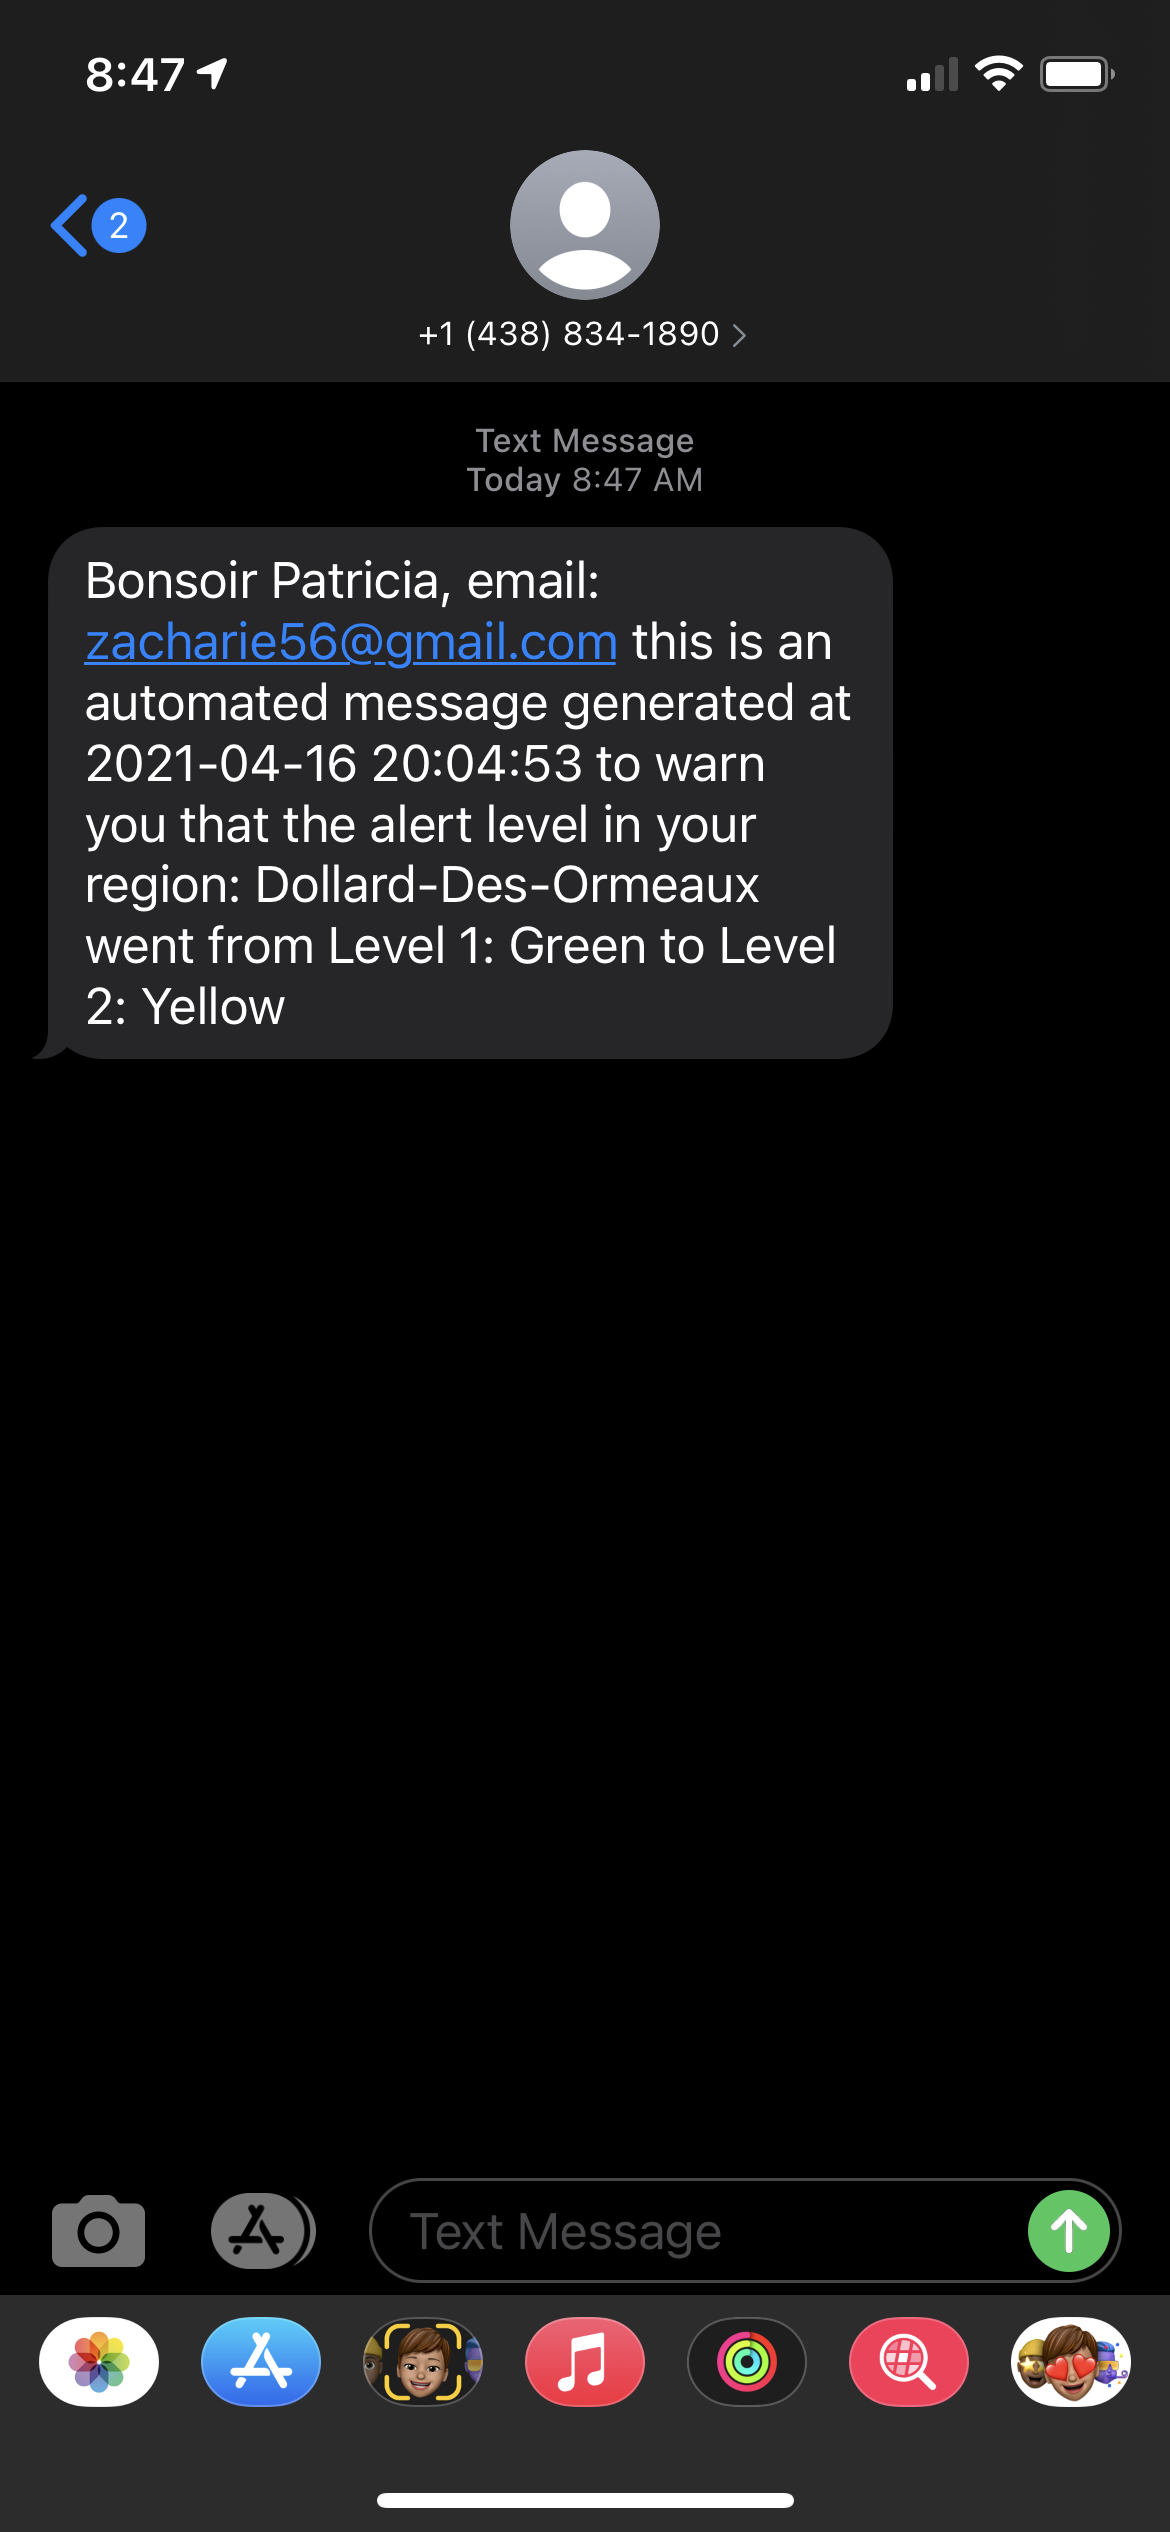
\includegraphics[scale=0.15]{imgs/sms.png}
    \caption{Our webapp sends text messages using the Twilio SMS API}
\end{figure}